% https://tex.stackexchange.com/a/343240
\documentclass{beamer}

\usepackage{tikz}
\usetikzlibrary{trees,positioning} 
\usetikzlibrary{matrix}            

\begin{document}


\begin{frame}[fragile]{Findings 3} 
\begin{block}{$\{ [\phi(h),p(t+h)]_C \}$}
  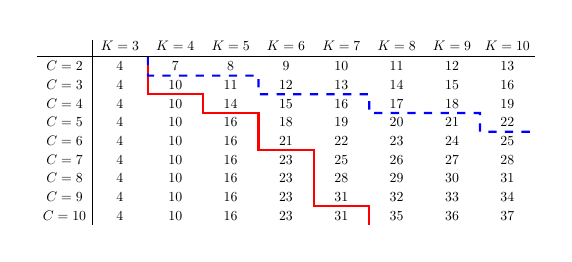
\begin{tikzpicture}[scale=0.5, every node/.style={scale=0.5}]
    \matrix (m)[%
          matrix of math nodes,
        column 1/.style={nodes={rectangle,minimum width=4em}},
        column 2/.style={nodes={rectangle,minimum width=4em}},
        column 3/.style={nodes={rectangle,minimum width=4em}},
        column 4/.style={nodes={rectangle,minimum width=4em}},
        column 5/.style={nodes={rectangle,minimum width=4em}},
        column 6/.style={nodes={rectangle,minimum width=4em}},
        column 7/.style={nodes={rectangle,minimum width=4em}},
        column 8/.style={nodes={rectangle,minimum width=4em}},
        column 9/.style={nodes={rectangle,minimum width=4em}},
        nodes in empty cells
    ]{
      & K=3 & K=4 & K=5 & K=6 & K=7 & K=8 & K=9 & K=10 \\
      \hline
      C=2   & 4   & 7   & 8   & 9     & 10    & 11    & 12    & 13 \\
      C=3   & 4   & 10  & 11  & 12    & 13    & 14    & 15    & 16 \\
      C=4   & 4   & 10  & 14  & 15    & 16    & 17    & 18    & 19 \\
      C=5   & 4   & 10  & 16  & 18    & 19    & 20    & 21    & 22 \\
      C=6   & 4   & 10  & 16  & 21    & 22    & 23    & 24    & 25 \\
      C=7   & 4   & 10  & 16  & 23    & 25    & 26    & 27    & 28 \\
      C=8   & 4   & 10  & 16  & 23    & 28    & 29    & 30    & 31 \\
      C=9   & 4   & 10  & 16  & 23    & 31    & 32    & 33    & 34 \\
      C=10  & 4   & 10  & 16  & 23    & 31    & 35    & 36    & 37 \\
    };
    \draw ([yshift=0.5em]m-1-1.north east) -- (m-10-1.south east);
        \only<2->{
            \draw[red,thick]
            (m-2-2.north east) --
            (m-3-2.south east) --
            (m-3-3.south east) --
            (m-4-3.south east) --
            (m-4-4.south east) --
            (m-6-4.south east) --
            (m-6-5.south east) --
            (m-6-5.south east) --
            (m-9-5.south east) --
            (m-9-6.south east) --
            (m-10-6.south east)
            ;
            \draw[blue,dashed,thick]
            (m-2-2.north east) --
            (m-2-2.south east) --
            (m-2-4.south east) --
            (m-3-4.south east) --
            (m-3-6.south east) --
            (m-4-6.south east) --
            (m-4-8.south east) --
            (m-5-8.south east) --
            (m-5-9.south east);
        }
    \end{tikzpicture}
\end{block}

\begin{block}{$\{ [\phi(h),p(t+h)]_C \}$}
  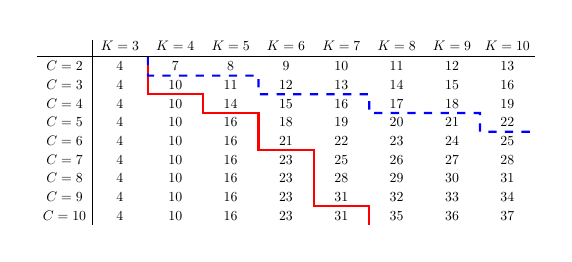
\begin{tikzpicture}[scale=0.5, every node/.style={scale=0.5}]
    \matrix (m)[%
          matrix of math nodes,
        column 1/.style={nodes={rectangle,minimum width=4em}},
        column 2/.style={nodes={rectangle,minimum width=4em}},
        column 3/.style={nodes={rectangle,minimum width=4em}},
        column 4/.style={nodes={rectangle,minimum width=4em}},
        column 5/.style={nodes={rectangle,minimum width=4em}},
        column 6/.style={nodes={rectangle,minimum width=4em}},
        column 7/.style={nodes={rectangle,minimum width=4em}},
        column 8/.style={nodes={rectangle,minimum width=4em}},
        column 9/.style={nodes={rectangle,minimum width=4em}},
        nodes in empty cells
    ]{
      & K=3 & K=4 & K=5 & K=6 & K=7 & K=8 & K=9 & K=10 \\
      \hline
      C=2   & 4   & 7   & 8   & 9     & 10    & 11    & 12    & 13 \\
      C=3   & 4   & 10  & 11  & 12    & 13    & 14    & 15    & 16 \\
      C=4   & 4   & 10  & 14  & 15    & 16    & 17    & 18    & 19 \\
      C=5   & 4   & 10  & 16  & 18    & 19    & 20    & 21    & 22 \\
      C=6   & 4   & 10  & 16  & 21    & 22    & 23    & 24    & 25 \\
      C=7   & 4   & 10  & 16  & 23    & 25    & 26    & 27    & 28 \\
      C=8   & 4   & 10  & 16  & 23    & 28    & 29    & 30    & 31 \\
      C=9   & 4   & 10  & 16  & 23    & 31    & 32    & 33    & 34 \\
      C=10  & 4   & 10  & 16  & 23    & 31    & 35    & 36    & 37 \\
    };
    \draw ([yshift=0.5em]m-1-1.north east) -- (m-10-1.south east);
        \only<2->{
            \draw[red,thick]
            (m-2-2.north east) --
            (m-3-2.south east) --
            (m-3-3.south east) --
            (m-4-3.south east) --
            (m-4-4.south east) --
            (m-6-4.south east) --
            (m-6-5.south east) --
            (m-6-5.south east) --
            (m-9-5.south east) --
            (m-9-6.south east) --
            (m-10-6.south east)
            ;
            \draw[blue,dashed,thick]
            (m-2-2.north east) --
            (m-2-2.south east) --
            (m-2-4.south east) --
            (m-3-4.south east) --
            (m-3-6.south east) --
            (m-4-6.south east) --
            (m-4-8.south east) --
            (m-5-8.south east) --
            (m-5-9.south east);
        }
    \end{tikzpicture}
\end{block}
\end{frame}

\end{document}
